%%%%%%%%%%%%%%%%%%%%%%%%%%%%%%%%%%%%%%%%%%%%%%%%%%%%%%%%%%%%%%%%%%%%%%%
%                          template.tex
%
% LaTeX template for papers conforming to the United States Sections of
% the Combustion Institue style guide.
%
% Authors:
%     Bryan W. Weber, University of Connecticut
%     Kyle E. Niemeyer, Oregon State University
%
% This work is licensed under the Creative Commons Attribution 4.0
% International License. To view a copy of this license, visit
% http://creativecommons.org/licenses/by/4.0/.
%%%%%%%%%%%%%%%%%%%%%%%%%%%%%%%%%%%%%%%%%%%%%%%%%%%%%%%%%%%%%%%%%%%%%%%
\documentclass[12pt]{ussci}

%======================================================================
\usepackage{todonotes}
\usepackage{graphicx}
\usepackage[binary-units]{siunitx}
\usepackage{gensymb}
\usepackage{amsmath}
\usepackage[version=3]{mhchem} % Formula subscripts using \ce{}, e.g., \ce{H2SO4}
\usepackage{booktabs,multicol} %better tables
\usepackage{subcaption} %subfigs
\sisetup{group-separator={,},
	detect-all,
	binary-units,
	list-units = single,
	range-units = single,
	range-phrase = --,
	per-mode = symbol-or-fraction,
	separate-uncertainty = true,
	multi-part-units = single,
	list-final-separator = {, and }
	%    scientific-notation = fixed
}
%======================================================================
% Add your bibliography file here, replace template.bib
\addbibresource{paper.bib}
%======================================================================
% Replace "Reaction Kinetics" in the line below by your paper topic
\newcommand\papertopic{Reaction Kinetics}
%======================================================================

\title{SIMD-vectorized Chemical Source Term Evaluation}

\author[*]{Nicholas Curtis}
\author[ ]{Chih-Jen Sung}

\affil[ ]{Department of Mechanical Engineering, University of Connecticut, Storrs, CT 06269, USA}
\affil[*]{Corresponding author: \email{nicholas.curtis@uconn.edu}}

\begin{document}
\maketitle

%====================================================================
\begin{abstract} % not to exceed 200 words
A code generation platform for single-instruction, multiple-data (SIMD) vectorized chemical source term evaluation was developed and validated against Cantera for a wide range of chemical kinetic models.
Speedups of up to \SIrange{1.88}{2.42}{$\times$} were observed over a baseline single-instruction, multiple-thread (SIMT) parallelized code.
Additionally, use of a row-major data layout was found to increase both the SIMD and SIMT performance by up to \SIrange{1.96}{2.38}{$\times$} over a column-major data layout.
Larger vector-widths were found to produce speedups up to \SI{1.8}{$\times$} as compared to a small vector-width for smaller models, e.g. GRI-Mech 3.0, but as the model size increased the performance of all vector-widths were similar.
Finally, the parallel scaling efficiency was found to be slightly better for larger models, and future extensions of this work were discussed.
\end{abstract}

% (Provide 2-4 keywords describing your research. Only abbreviations firmly
% established in the field may be used. These keywords will be used for
% sessioning/indexing purposes.)
\begin{keyword}
    Chemical Kinetics\sep SIMD \sep Vector Processing
\end{keyword}

%====================================================================
\section{Introduction}
%

Single-Instruction, Multiple-Data (SIMD) processing, also known as vector-processing, is an important parallel computing paradigm used increasingly in scientific computing.
Traditional multi-core parallelism is often used to increase central processing unit (CPU) performance, however SIMD processors---and the related Single-Instruction, Multiple-Thread (SIMT) processors, e.g. graphics processing units (GPUs)---have gained recognition due to their increased floating operation throughput.
The parallel programming standard OpenCL~\cite{stone2010opencl} has further enabled adoption of vector-processing based codes in scientific computing by providing a common application program interface (API) for execution on heterogeneous systems (e.g. CPU, GPU, etc.).

\begin{figure}[htb]
  \centering
  \begin{subfigure}[t]{0.45\linewidth}
      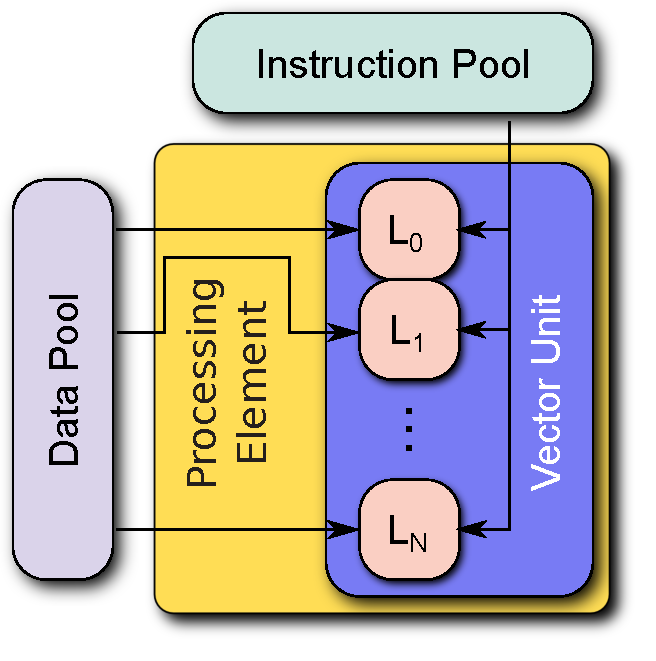
\includegraphics[width=\textwidth]{SIMD.pdf}
      \caption{Schematic of SIMD processing.  A single processing element (e.g. a CPU core) contains a vector unit with several lanes (L0, L1, etc.).  The vector unit executes a single instruction concurrently on multiple data.}
      \label{F:SIMD}
  \end{subfigure}
  \hfill
  \begin{subfigure}[t]{0.45\linewidth}
      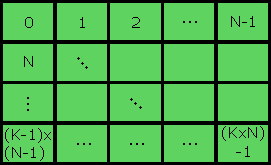
\includegraphics[width=\textwidth]{mem_access.pdf}
      \caption{Representation of an 2-D array with dimension $N_1 \times N_2$ in CPU memory, with linear index marked.}
      \label{F:mem}
  \end{subfigure}
\end{figure}

A SIMD instruction utilizes specialized vector processing hardware to execute the same floating point operation (e.g. multiplication, division, etc.) on a several different data concurrently (Fig.~\ref{F:SIMD}); the number of concurrent operations is known as the vector-width\footnote{OpenCL allows for use of vector-widths not equal to the hardware vector-width via implicit conversion, and may provide some performance benefit as will be studied here}.
Nearly all modern CPUs have vector processing units capable of running SIMD instructions, typically capable of handling 2--4 concurrent double precision operations.
Additionally, specialized hardware accelerators, e.g. Intel's Xeon Phi co-processor (or MIC), have been developed that have tens of cores with very wide vector widths (e.g. 4--8 double precision operations); these very wide vector widths are also expected on forthcoming Intel CPUs (the Skylake Xeon and Cannon Lake architectures).

\subsection{Data ordering and vectorization patterns}
\label{S:data}
When storing arrays for a chemical kinetic model, e.g. the concentration of species $k$ for the $j$-th of thermo-chemical state $[C_k]_j$ there are two data-ordering choices.
In the ``F'' (Fortran column-major) format, the concentrations of a single species $k$ over all $N$ thermo-chemical states are adjacent.
In Fig.~\ref{F:mem} this would correspond to storing $[C_0]_0$ in index \num{0}, $[C_0]_1$ in index \num{1} and so on, with $N_1 = N$, and $N_2 = N_s$, the number of species in the model.
In the ``C'' (C row-major) format, the storage order is transposed with $[C_0]_0$ in index \num{0}, $[C_1]_0$ in index \num{1} etc., and $N_1 = N_s$, $N_2 = N$.
This ordering---along with the device (CPU, GPU, etc.) in question---have a large effect on the performance of SIMD\slash SIMT-vectorized algorithms.

In a \textit{shallow}-SIMD vectorization, each SIMD-lane evaluates chemical source terms for a different thermo-chemical state.
If the data is stored in ``F''-order, the SIMD-lanes accessing the concentration of species $k$ for states $j, j+1\ldots$ will load sequential locations in memory, however the $k+1$th species concentration will be $N$ memory locations away increasing the likelihood of cache-misses on the CPU.
In a \textit{deep}-SIMD vectorization, a vector-unit cooperates to evaluate chemical source terms for a single thermo-chemical state $j$, thus SIMD-lanes loading species concentrations $k, k+1\ldots$ will access sequential memory locations if the data is stored in ``C''-order.
Further, in the ``C''-ordering the furthest difference between any two concentrations in a single thermo-chemical state is at most $N_s$, with $N_s \ll N$ in most cases; this greatly improved data-locality increases the chances of a cache-hit on the CPU.
However, a deep vectorization may result in SIMD-\textit{waste}---similar to thread-divergence in GPU-processing---caused by different SIMD-lanes executing different instructions (e.g. from differing for-loop bounds).

Finally, in a SIMT-vectorization, threads execute the same instruction over multiple data in lock-step without use of specialized vectorization instructions.
This is the paradigm used in GPU-processing, a more through review of which can be found in our previous work~\cite{CurtisGPU:2017}; one key-exception in this case is that the algorithm executed to evaluate the chemical source terms is identical for all thermo-chemical states, thus there is no thread-divergence for a shallow SIMT-vectorization. 
In Sec.~\ref{S:results} the effect of the data-ordering on the shallow-SIMD\slash SIMT vectorization performance will be studied.

\subsection{Previous works and goals of this study}
Several recent works, e.g. \cite{CurtisGPU:2017} have investigated SIMT-based chemical kinetic integration on GPUs, however SIMD-based chemical kinetics have been less studied in comparison.
\textcite{stone2016} implemented a linearly-implicit fourth-order stiff Rosenbrock solver in the OpenCL for various platforms including the CPU, GPU and the MIC.
The shallow-SIMD and SIMT-vectorization models were implemented in OpenCL and compared to an OpenMP baseline code that was deep SIMD-vectorized by simple compiler hints (a.k.a pragmas).
The shallow-SIMD vectorization improved the integrator performance over the OpenMP baseline by \SIrange{2.5}{2.8}{$\times$} on the CPU and \SIrange{4.7}{4.9}{$\times$} on the MIC, while the GPU performance was \SIrange{1.4}{1.6}{$\times$} slower than the OpenMP baseline due to thread-divergence concerns.
\textcite{kroshko2013efficient} implemented a shallow-SIMD vectorized third order stiff Rosenbrock integrator for atmospheric chemistry on a Cell Broadband Engine---a specially designed vector processor---finding a speedup of \SI{1.89}{$\times$} over a serial version of the same code, a \SI{94}{\percent} parallel efficiency.

This work will study the performance of chemical source term evaluation of automatically generated shallow-SIMD vectorized codes for a wide range chemical kinetic models on the CPU.
The performance will be compared to a baseline shallow-SIMT vectorized code to determine the effective SIMD speedup.
Finally future extensions to this work will be detailed.

\section{Methodology}
\subsection{Chemical Kinetics Equations}
The current code evaluates the following chemical source terms:

\begin{equation}
\frac{\text{d}[C_k]}{\text{d}t} = \sum_{i}^{N_R} \nu_{k,i} R_i c_i
\end{equation}
where $\frac{\text{d}[C_k]}{\text{d}t}$, $N_R$, $\nu_{k,i}$, ${R_i}$, $c_i$ are the time rate of change of the concentration of species $k$, the number of reactions in the model, the net stoichiometric coefficient of species $k$ in reaction $i$, the net rate of progress of reaction $i$, and the pressure modification of reaction $i$ respectively.
For further detail on each term, the reader is referred to our previous work~\cite{Niemeyer:2016aa}; the code is capable of evaluating all modern reaction rate types (e.g. pressure-log, chebyshev, etc.).

In addition, the temperature rate of change using the constant-pressure assumption\footnote{Note: in this context, the ``constant-pressure assumption'' refers to evaluation within a reaction sub-step in the operator splitting scheme, rather than a general constant-pressure reactive-flow simulation.} is evaluated as:
\begin{equation}
\frac{\text{d}[T]}{\text{d}t} = -\frac{\sum_{k}^{N_S} H^{\degree}_k \frac{\text{d}[C_k]}{\text{d}t}}{\sum_{k}^{N_S} [C_k] c_{p_k}^{\degree}}
\end{equation}
where $H^{\degree}_k$ and $c_{p_k}^{\degree}$ are the molar specific enthalpy and specific heat respectively.
Although the code is equally capable of a evaluating the temperature rate using a constant-volume assumption, we omit this here for brevity.

\subsection{Code Generation}
Code generation is enabled by the python package \texttt{loo.py}~\cite{kloeckner_loopy_2014}, which translates user specified psuedo-code and data to OpenCL, allowing for unit testing and easy changes of program structure, e.g. data ordering, vectorization, threading patterns etc.

\section{Results and Discussion}
\subsection{Validation}
The reaction rates of progress (ROP), species and temperature rates in this study are validated by comparison with Cantera~\cite{Cantera}, however special care must be taken due floating point arithmetic issues

In computing the net ROP of reaction $i$ from the forward and reverse ROP: $R_{i} = R_{i}^{\prime} - R_{i}^{\prime\prime}$, precision can easily be lost as the net ROP may be---particularly near chemical equilibrium---many orders of magnitude smaller than the forward or reverse rates.
A base-ten bound on loss of precision~\cite{goldberg1991every} can be found as:
\begin{equation}
\text{L}_{i,\text{min}} = 2^{-p_i} \le \left\lvert 1 - \frac{R_{i}^{\prime}}{R_{i}^{\prime\prime}} \right\rvert \le 2^{-q_i} = \text{L}_{i,\text{max}}}
\label{e:bounds}
\end{equation}
with $q_i \le p_i$.
To obtain an estimate of the precision bounds, the forward and reverse ROP from Cantera are substituted into Eq.~\eqref{e:bounds}.
Additionally a higher-precision number format (in this case, the Python Decimal class) is used in this computation to maintain accuracy.
Finally, when determining the error in the net ROP between this code and Cantera, the bounds on the percent error attributable to precision loss, $\text{P}_{i,\text{err}}$ can be estimated as:
\begin{equation}
\text{P}_{i,\text{min}} = 100 * \frac{\text{L}_{i,\text{min}}}{\left\lvert\ R_{i,\text{CT}} - R_{i}\right\rvert} \le
\text{P}_{i,\text{err}} \le 100 * \frac{\text{L}_{i,\text{max}}}{\left\lvert R_{i,\text{CT}} - R_{i} \right\rvert} = \text{P}_{i,\text{max}}
\label{e:rel_bound}
\end{equation}
where the \text{CT} subscript indicates values from Cantera.

For a more direct comparison, a relative error norm of a quantity $X_{i,j}$ over all states $j$, and indices $i$ was computed using the $L^{\infty}$ norm:
\begin{equation}
 E_{X_{i}} = \left\lVert \frac{\left\lvert X_{i,j,\text{CT}} - X_{i,j}\right\rvert}{\num{e-10} + \num{e-6} * \left\lvert X_{i,j,\text{CT}} \right\rvert} \right\rVert_{i,j,\infty}
\label{e:rel_err}
\end{equation}
and the lower precision bound for the net ROP error norm is set to $\text{P}_{\text{min}}^{*} = \text{P}_{i,\text{min}}$ for the $i, j$ value that results in the maximum error $E_{R_i}$.

\begin{table}[htb]
\sisetup{retain-zero-exponent=true}
\centering
\begin{tabular}{@{}S[table-format=1.2e1] S[table-format=1.2e1] S[table-format=1.2e1] S[table-format=1.2e1] S[table-format=1.2e1] S[table-format=1.2e1] S[table-format=1.2e1] @{}}
\toprule
\multicolumn{1}{l}{Model} & \multicolumn{1}{c}{$E_{R_{i}^{\prime}}$} & \multicolumn{1}{c}{$E_{R_{i}^{\prime\prime}}$} &\multicolumn{1}{c}{$E_{R_{i}}$} & \multicolumn{1}{c}{$\text{P}_{\text{min}}^{*}\si{\percent}$} & \multicolumn{1}{c}{$E_{\frac{\text{d}[C_k]}{\text{d}t}}$} & \multicolumn{1}{c}{$E_{\frac{\text{d}[T]}{\text{d}t}}$} \\
\midrule
\multicolumn{1}{l}{\ce{H2}\slash~\ce{CO}\cite{Burke:2011fh}} & 1.20e-8 & 6.33e-8 & 1.32e1 & 4.66e6 & 2.37e1 & 2.12e5 \\
\multicolumn{1}{l}{GRI-Mech.~3.0\cite{smith_gri-mech_30}}  & 3.07e-8 & 5.90e-8 & 1.21e0 & 2.67e04 & 2.84e0 & 2.64e4 \\
\multicolumn{1}{l}{USC-Mech II\cite{Wang:2007}}  & 1.07e-7 & 1.37e-7 & 2.39e0 & 4.12e02 & 7.92e00 & 3.22e03 \\
\multicolumn{1}{l}{\ce{IC5H11OH}\cite{Sarathy:2013jr}} & -1 &  -1 & -1 & -1 & -1 & -1 \\
\bottomrule
\end{tabular}
\caption{Summary of rate of progress, species and temperature rate correctness.
Error statistics are based on the infinity-norm of the relative error detailed in Eq.~\eqref{e:rel_err} for each quantity.
\todo[inline]{i-pentanol validation still running}
}
\label{T:error}
\end{table}

In Table~\ref{T:error}, we see the results of this code as compared to Cantera on a library of partially stirred reaction conditions (PaSR) described in our previous works~\cite{CurtisGPU:2017,Niemeyer:2016aa}.
Very close agreement is observed for the forward and reverse ROP for all models, however the net ROP error norm is \numrange{7}{8} orders of magnitude larger.
We see here that the minimum estimated loss of precision is \SIrange{4}{40}{$\times$} the error in net ROP, explaining this jump.
The species rate error norm is similar in magnitude to that of the net ROP, however the temperature rate error again increases as it depends directly on the species rates.
We note that the above discussion does not imply that computation of the net ROP will cause large error in chemical kinetic integration---either in this code or Cantera---as this loss of precision only occurs when the forward and reverse ROP are nearly equal, implying the reaction is in near-equilibrium.

\subsection{Results}
\label{S:results}
The performance studies in this work were run on four ten-core \SI{2.2}{\giga\hertz} Intel Xeon E5-4640 v2 CPUs with \SI{20}{\mega\byte} of L3 cache memory, installed on an Ace Powerworks PW8027R-TRF+ with a Supermicro X9QR7-TF+/X9QRi-F+ baseboard.
Runtimes in each case were averaged over ten runs, each using the same set of PaSR conditions utilized in validation.
All code was compiled with \texttt{gcc 4.8.5} and ``\texttt{-O3}'' optimization, running on \texttt{v16.1.1} of the Intel OpenCL runtime supporting OpenCL \texttt{v1.2}.

\begin{figure}[htb]
  \centering
  \begin{subfigure}[t]{0.48\textwidth}
    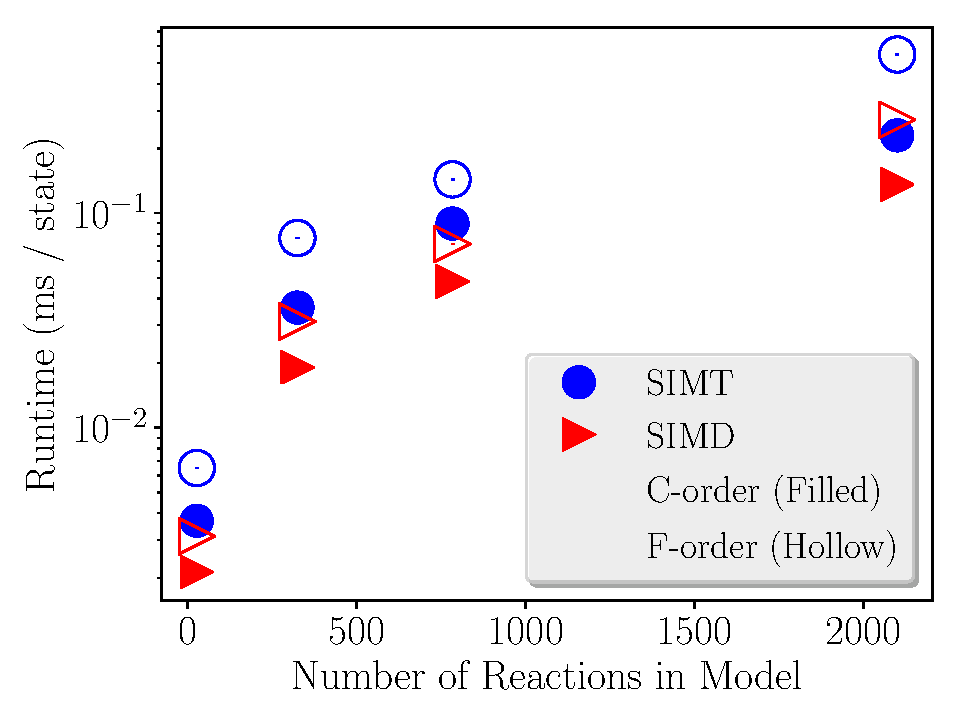
\includegraphics[width=\textwidth]{SIMD_SIMT_Order_comparison}
    \caption{Runtime in milliseconds per thermo-chemical state of shallow-SIMD and SIMT-vectorization on a single CPU core for both ``C'' (filled symbols) and ``F'' (empty symbols) data ordering.}
    \label{F:SIMDComp}
  \end{subfigure}
  \hfill
  \begin{subfigure}[t]{0.48\textwidth}
    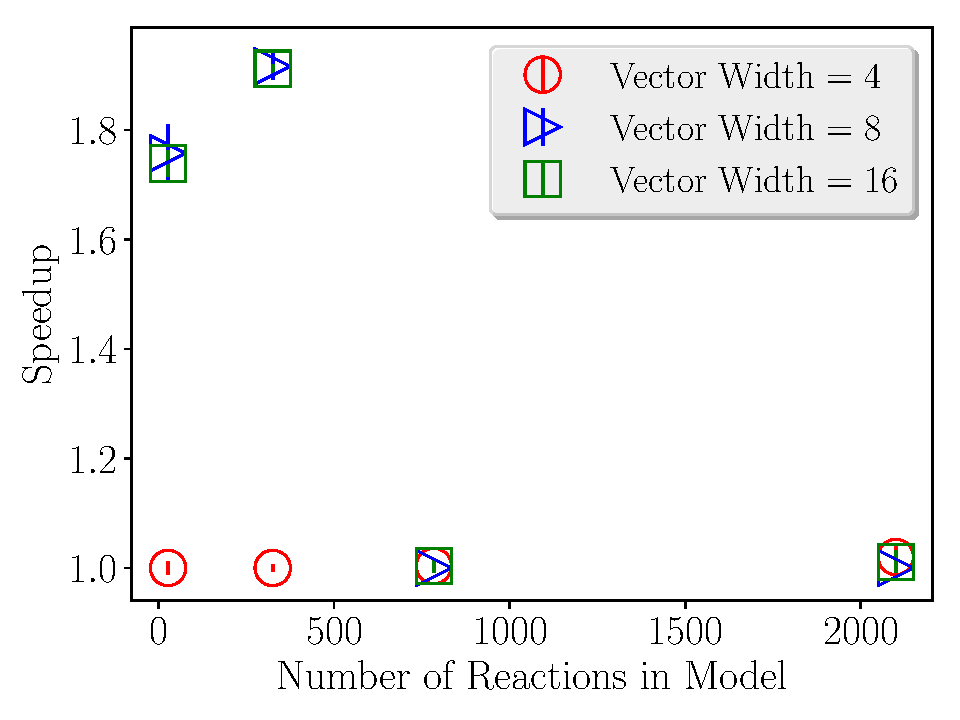
\includegraphics[width=\textwidth]{SIMD_Vecwidth_comparison}
    \caption{Speedup of a ``C''-ordered shallow-SIMD vectorization on a single CPU core when varying the supplied vector-width.}
    \label{F:Veccomp}
  \end{subfigure} \\
  \begin{subfigure}[t]{0.5\textwidth}
    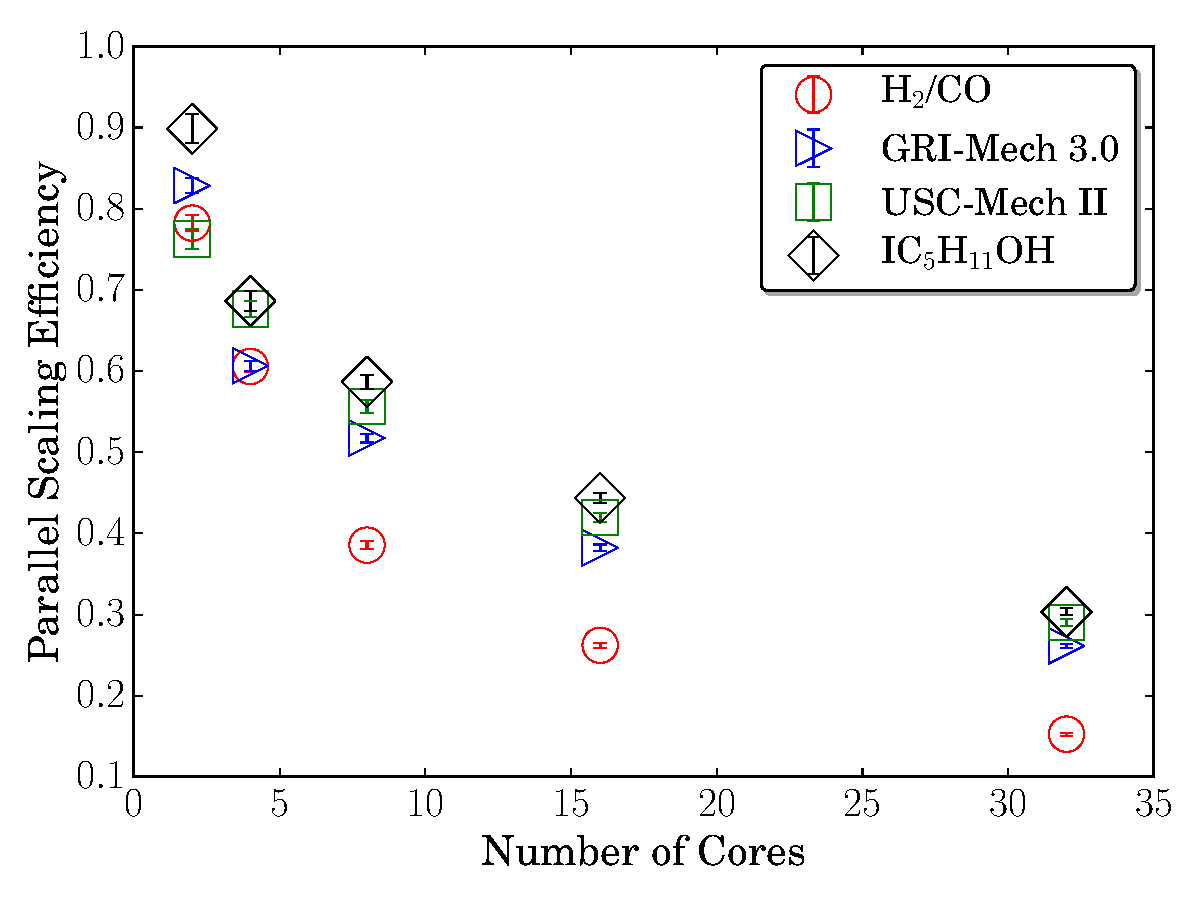
\includegraphics[width=\textwidth]{SIMD_scaling}
    \caption{Strong parallel scaling of a ``C''-ordered shallow-SIMD vectorization using a vector width of 16.}
    \label{F:SIMDscale}
  \end{subfigure}
\end{figure}

In Fig.~\ref{F:SIMDComp}, the performance of the shallow-SIMD and SIMT vectorization are compared on a single CPU core for both ``C'' and ``F'' memory formats.
The ``C''-ordered SIMD\slash SIMT vectorizations show a speedup over the equivalent ``F''-ordered code by \SIrange{1.36}{1.96}{$\times$} and \SIrange{1.60}{2.38}{$\times$} respectively.
This demonstrates that enhanced data-locality of the ``C''-ordering for CPU caching---discussed in Sec.~\ref{S:data}---is key to high performance on the CPU, and suggests that a deep vectorization would see even greater accelerations.
The shallow vectorization is consistently faster than the SIMT vectorization, by \SIrange{1.72}{1.88}{$\times$} and \SIrange{2.10}{2.42}{$\times$} for the ``C'' and ``F'' memory formats respectively.
This is less than the theoretical maximum speedup on this CPU, which can process \SI{256}{\bit} AVX instructions (i.e. four double-precision operations) concurrently.
Most likely this is due to the non-sequential memory access patterns of the shallow vectorization discussed previously, but could also be caused in part by inefficiencies in translation of the OpenCL code to AVX code, a process handled by the Intel Opencl Runtime.

The effect of changing the vector-width supplied to a ``C''-ordered shallow-SIMD vectorization on a single CPU core is investigated in Fig.~\ref{F:Veccomp}.
Significant speedups are seen with larger vector-widths for the smaller models, however as the model size increases data must be loaded from increasingly distant memory locations and the performance of all three vector widths becomes similar.
Finally in Fig.~\ref{F:SIMDscale} the strong parallel scaling of the chemical source term evaluation is examined for all four models with a ``C''-ordered shallow SIMD-vectorization and vector-width of 16:
Interestingly the efficiency for the hydrogen model decreases fastest, while the larger models have similar efficiencies; the isopentanol model has the highest efficiency in all cases.
This suggests that evaluation of the chemical-source terms for a single thermo-chemical state for the smaller models may not saturate the processing power of the CPU, some efficiency may be lost due to context switching within OpenCL itself.
Additionally, OpenCL allows assigning of work to devices by shared memory resources e.g., a L3 cache, which was not pursued in this study for simplicity; this should be investigated in future work to determine the effect on scaling efficiency.

\section{Conclusions}
In this work, a shallow SIMD-vectorized chemical source term evaluation OpenCL code generator was developed and validated against Cantera~\cite{Cantera} for a wide range of chemical kinetic models~\cite{Burke:2011fh,smith_gri-mech_30,Wang:2007,Sarathy:2013jr}.
Significant speedups of up to \SIrange{1.88}{2.42}{$\times$} over a baseline SIMT-vectorized code were observed.
Two data-ordering schemes were investigated, showing a clear performance benefit for use of the ``C'' (row-major) ordering for the shallow vectorized code.
Further, this study suggests that a deep SIMD-vectorized code---currently under development---may see even greater accelerations due to expected increases in cache-hit rates.
Larger vector widths were found to provide accelerations for the smaller models studied, but performance was similar over all vector widths tested for the largest models tested.
Finally, the strong parallel scaling efficiency was examined for the shallow vectorized code; the larger models exhibited higher scaling efficiency, possibly due to failure of the \ce{H2}\slash\ce{CO} model to saturate the CPU throughput.
Future extensions of this work will include development of a SIMD\slash SIMT-accelerated sparse-analytical Jacobian code targeted at CPUs, GPUs and MICs.

\section{Acknowledgements}
This research was funded by \ldots

\printbibliography[heading=bibintoc]

\end{document}
